\documentclass[12pt,a4paper]{article}
\usepackage[margin=2cm]{geometry}
\usepackage[main=italian]{babel}
\usepackage{amssymb,amsmath}
\usepackage{graphicx}
\graphicspath{ {./img/} }
\usepackage{float}
\floatplacement{figure}{H}
\usepackage[export]{adjustbox}
\usepackage{caption}
\usepackage{subcaption}
\usepackage{enumitem}
\usepackage{hyperref}
\usepackage{pgfplots}
\pgfplotsset{compat=1.18}

\makeatletter
\renewcommand*{\p@subsection}{\thesection.}
\makeatother

\begin{document}
\title{\textbf{Studio della mobilità terra-mare a Rimini}}
\author{Gregorio Berselli, Luca Ferragina}
\date{}
\maketitle

\begin{abstract}
In questo studio si vuole verificare la correlazione tra diverse grandezze fisiche di interesse nella mobilità usando come riferimento alcuni dati della città di Rimini.
Una volta suddivisa l'area di interesse in una griglia di 380 $\times$ 380 celle, ciascuna corrispondente a una superficie di circa 3.5 km\textsuperscript{2}, e rimossi i dati ritenuti rumore, si sono studiati gli andamenti di densità di popolazione / distanza, distanza / tempo e velocità / tempo.
Dalle analisi precedenti si è inoltre ricavata la dipendenza della velocità dalle densità.
L'ipotesi di partenza prevede di poter descrivere la mobilità, in buona approssimazione, come quella di particelle soggette ad un campo di forze e i risultati ottenuti sono compatibili con le attese.
\end{abstract}

\section{Introduzione}
L'idea di partenza per questo studio è quella di verificare l'applicabilità di un modello stile deep gravity alla mobilità umana, in modo da descrivere in maniera relativamente semplice e, soprattutto, dipendente da pochi parametri tutti i processi complessi che governano la mobilità all'interno delle città.
Secondo un modello di questo tipo è possibile schematizzare il movimento delle persone all'interno di una città in maniera simile a quello che avrebbero delle particelle immerse in un potenziale gravitazionale.
Naturalmente, non si cerca di indagare sui dettagli degli spostamenti, come la scelta del percorso, ma è possibile risalire ad alcuni parametri medi rilevanti nello studio della mobilità ai fini, ad esempio, di analisi statistiche, di traffico o per cercare di prevedere possibili zone con frequentazione molto superiore alla media, che diventano degli attrattori gravitazionali. \\
Volendo studiare la mobilità cittadina e avendo a disposizione dati relativi ad alcune giornate estive registrati nella città costiera di Rimini, ci si è interessati nello specifico ai movimenti tra la parte interna della città e la zona più vicina al mare, che risulta quindi un attrattore, in modo da minimizzare il ``rumore'' proveniente dalla vicina autostrada, naturalmente soggetta ad una mobilità estremamente diversa.
Lo studio si è concentrato sugli aspetti più semplici, andando a cercare proprietà medie descrivibili, come la distribuzione della densità di persone che hanno eseguito un certo viaggio in funzione della distanza percorsa o della velocità media durante il viaggio e la distanza percorsa o la velocità media in funzione del tempo di percorrenza.
Per portare avanti questo studio si è considerato un articolo che si prefiggeva finalità simili \cite{Mobility}.
Dall'articolo usato come guida sono stati estrapolati alcuni dei risultati attesi, come l'andamento tipico a potenza che dovrebbe seguire la densità di persone in funzione della distanza e gli andamenti a potenza delle altre grandezze in analisi, tenendo comunque conto della differenza sia nei dati a disposizione che nella metodologia.

\section{Modello teorico e svolgimento}
\begin{figure}
\centering
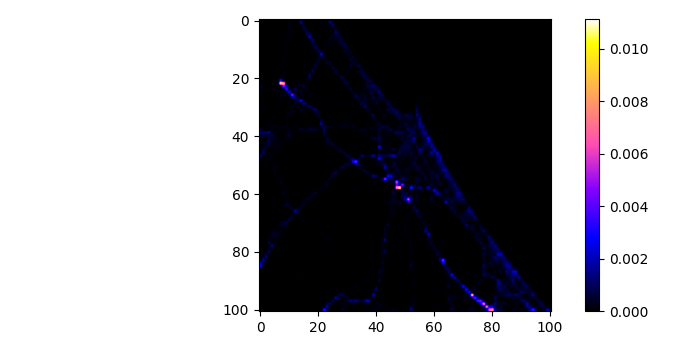
\includegraphics[width=\textwidth]{init.png}
\caption{\emph{Esempio di suddivisione della mappa in 100 $\times$ 100 celle in modo da favorirne la visualizzazione. La scala cromatica rappresenta la densità di agenti.}}
\label{figure:cells}
\end{figure}
Step fondamentale del modello teorico è la suddivisione dell'area studiata in celle.
L'intera area considerata è stata quindi suddivisa in 380 $\times$ 380 celle (si veda esempio in Fig. \ref{figure:cells}), ognuna delle quali ricopre una superficie di circa $3.5$ km\textsuperscript{2}.
Successivamente, è stato utilizzato un codice Python per isolare i singoli soggetti tracciati e organizzarne i dati, in modo tale da poter disegnare i grafici.
In particolare, per ogni individuo, caratterizzato da un codice univoco, sono state separate le coordinate iniziali e finali (in lat-long), il tempo di tracciamento, distanza reale e distanza in linea d'aria percorse (in km).
Tramite un altro script Python è poi stato definito un filtro terra/mare per distinguere le due zone di Rimini di interesse, prendendo come retta di separazione la ferrovia Adriatica.
Con questa considerazione si evita l'interferenza con il flusso autostradale, di interesse nullo in quanto non rilevante per la mobilità della città.\\
Una volta effettuata la distinzione sono poi stati estrapolati i dati graficati e studiati nella sezione successiva.
\begin{figure}[h!]
\centering
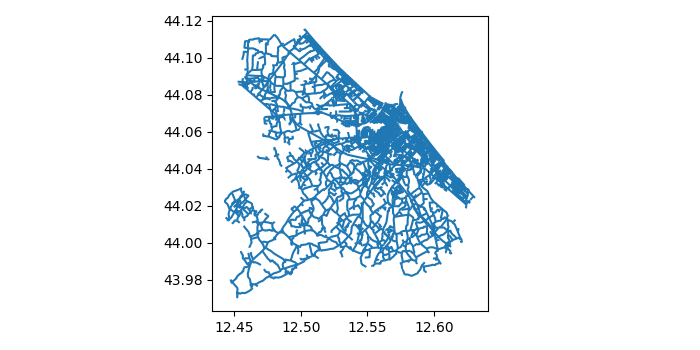
\includegraphics[width=0.75\textwidth]{city.png}
\caption{\emph{Network stradale della città di Rimini.}}
\label{figure:rimini}
\end{figure}

I dati a disposizione per l'analisi, forniti da TIM, riguardano la città di Rimini e le zone limitrofe nell'arco temporale che va dal 10/08/2020 al 16/08/2020, in piena stagione estiva.
Essendo questo uno studio sulla mobilità, i dati raccolti dipenderanno fortemente dal network stradale della stessa città di Rimini, riportato in Fig. \ref{figure:rimini}.
Come tutte le dinamiche su network ci si aspettano, in generale, osservabili del sistema legati tra loro da leggi a potenza.
Tuttavia, per le piccole distanze, avendo una mobilità prevalentemente pedonale, si tende a perdere l'influenza del network stradale (a piedi è spesso conveniente ``tagliare'' strada, quindi ignorare il network stesso).
Quest'ultimo fatto risulta evidente anche osservando il problema da un punto di vista puramente matematico: per $r\to 0$ una legge del tipo $r^\alpha$ perde evidentemente di validità per $\alpha<0$.
Risulta quindi ragionevole aspettarsi che, per piccole distanze, la città perda lo stato di attrattore e i moti al suo interno siano approssimabili a random walk.
\section{Risultati e discussione}
Le quattro correlazioni in esame hanno naturalmente forme e risultati attesi differenti, quindi ne separeremo la trattazione per chiarezza.
In tutti i casi vengono trascurate le costanti di normalizzazione delle curve, data l'invarianza di scala intrinseca delle leggi a potenza.

\subsection{Densità e distanza}
Per un flusso di persone come quello studiato è ragionevole ipotizzare che la densità di popolazione decresca all'aumentare della distanza percorsa.
Ci si aspetta, infatti, che un soggetto sia meno intenzionato a muoversi verso il mare tanto più è lontano da esso in quanto necessita di mezzi propri, viene coinvolto nel traffico, ecc.\\
Tuttavia, questa decrescita sarà a sua volta influenzata dal tipo di mobilità presa in considerazione: un gruppo di persone che si muove a piedi tende a comportarsi come un gas ideale (di Boltzmann), quindi ci si aspetta un decadimento di tipo esponenziale.
Una mobilità con mezzi motorizzati, come autobus o automobili, invece, risulta meglio descritta da un andamento a potenza.
Per ogni cella appartenente alla sezione del mare si è quindi studiata la quantità di persone dirette verso essa e provenienti da una cella della sezione terra in funzione della distanza.
Unendo poi i risultati ottenuti per tutte le celle del mare si è ottenuto il seguente grafico:
\begin{figure}[H]
\centering
\begin{tikzpicture}
\begin{axis}[
grid = both,
major grid style = {lightgray},
minor grid style = {lightgray!25},
width = 0.75\textwidth,
height = 0.5\textwidth,
xmode = log,
ymode = log,
xmax=10000,
ylabel near ticks,
xlabel near ticks,
xlabel = {Distanza percorsa ($m$)},
ylabel = {Densità di popolazione},]
\addplot[
domain = 200:3000,
samples = 200,
smooth,
thick,
blue,] {0.983136*exp(-0.000271663*x)};
\addplot[
domain = 3001:10000,
samples = 200,
smooth,
thick,
blue,] {1111.17*x^(-0.977487)};
\addplot[
mark size=0.69,
draw=black,
only marks,] file {./real_distance.dat};
\end{axis}
\end{tikzpicture}
\caption{\emph{Densità di popolazione in relazione alla distanza percorsa.}}
\label{figure:dens_dist}
\end{figure}
In Fig. \ref{figure:dens_dist} si osserva il cambiamento di mobilità ipotizzato con una distanza percorsa limite tra i due andamenti di circa $3$ km, perfettamente in accordo con le dimensioni della città di Rimini.
Nella figura è infatti riportato il fit dei dati eseguito con due funzioni differenti, discontinue proprio nella distanza limite.
La funzione ottenuta tramite il fit assume dunque la forma:      
\begin{equation}
\rho(r)\propto
\begin{cases}
e^{-0.00027 r} \quad &r<3\cdot 10^3$ m$\\
\frac{1}{r} \quad &3\cdot 10^3$ m$< r < 10^4$ m$
\end{cases}
\label{equation:rho_r}
\end{equation}
In questo modo si ottengono risultati in linea con le attese: 
\begin{itemize}
\item Per distanze inferiori a $3$ km l'andamento è descritto da una funzione esponenziale con esponente $\sim - 0.00027$ m$^{-1}$, il che ricorda un moto di tipo diffusivo;
\item A distanze superiori, che supponiamo non essere percorse a piedi, otteniamo un moto descritto da un andamento a potenza con esponente $\beta = -0.98$.
\end{itemize}
Un'ulteriore interpretazione di questo andamento si può ritrovare considerando la distribuzione in Eq. (\ref{equation:rho_r}) come la densità di popolazione di Rimini in funzione della distanza, la quale si riduce, come atteso, seguendo una legge a potenza.
Si noti ora come l'esponente della potenza è $\sim -1$ ma la funzione risulti egualmente normalizzabile in quanto definita per grandi valori della distanza.
La transizione di fase che permette il passaggio da legge esponenziale a potenza è tipica dei network complessi, il che è coerente con la problematica analizzata avendo soggetti che si muovono su un network stradale.
Anche il modello a potenza perde di validità per distanze superiori ai $10$ km ma possiamo trascurare questo problema in quanto il range considerato è già abbastanza esteso oltre la città di Rimini.\\

Risulta ora interessante ricavare la probabilità che un singolo individuo decida di effettuare un viaggio verso il mare, in relazione alla sua distanza da esso.
In tal caso, bisogna considerare l'intera popolazione che si trova nella zona terrestre e non solo coloro che hanno effettivamente intrapreso un viaggio verso la zona marina.
Viene immediato ipotizzare una distribuzione di probabilità nella forma:
\begin{equation}
    f(r)=\frac{n_{ttm(r)}}{n_{tot}(r)}
    \label{equation:frequenza}
\end{equation}
dove $f$ è la frequenza, $n_{ttm}$ il numero di individui in moto dalla terra al mare e $n_{tot}$ il numero totale di individui.
Come da considerazioni precedenti ci si aspetta che $f(r)$ sia una funzione decrescente con la distanza in quanto all'aumentare di essa lo ``sforzo'' compiuto dal soggetto per mobilitarsi risulta maggiore.
\begin{figure}[H]
\centering
\begin{tikzpicture}
\begin{axis}[
grid = both,
major grid style = {lightgray},
minor grid style = {lightgray!25},
width = 0.75\textwidth,
height = 0.5\textwidth,
xmode = log,
ymode = log,
ylabel near ticks,
xlabel near ticks,
xlabel = {Distanza percorsa ($m$)},
ylabel = {Probabilità di spostamento},]
\addplot[
domain = 100:3200,
samples = 200,
smooth,
thick,
blue,] {0.400803*exp(-0.000509662*x)};
% 2.452916 0.000238
\addplot[
domain = 3190:10000,
samples = 200,
smooth,
thick,
blue,] {7107860*(x+145)^(-2.25802)};
% 0.00153287 1.28
\end{axis}
\end{tikzpicture}
\caption{\emph{Probabilità che un individuo effettui un viaggio vesro il mare in relazione alla distanza percorsa.}}
\label{figure:frequenza}
\end{figure}
In Fig. \ref{figure:frequenza} si può notare come l'andamento sia coerente con l'ipotesi effettuata nell'Eq. (\ref{equation:frequenza}).
Dal fit si ottiene infatti la funzione
\begin{equation}
f(r)\propto
\begin{cases}
e^{-0.0005 r} \quad &r<3\cdot 10^3$ m$\\
\frac{1}{r^2} \quad &3\cdot 10^3$ m$ < r < 10^4$ m$
\end{cases}
\label{equation:f(r)}
\end{equation}
Si nota immediatamente come questa funzione rimanga di fatto costante per piccole distanze (l'esponente è in buona approssimazione nullo), in quanto essendo in piena stagione estiva la probabilità che un abitante di Rimini vada al mare è massima, poi decresca con la distanza con una potenza $\sim -2$.

\subsection{Distanza e tempo}
Anche la distanza e il tempo sono correlati tuttavia, in questo caso, conviene considerare la distanza distanza totale percorsa a partire dall'istante iniziale.
Secondo tale considerazione, l'andamento previsto è quello di una potenza: proprietà derivante dalla struttura a network del problema considerato.
\begin{figure}[H]
\centering
\begin{tikzpicture}
\begin{axis}[
grid = both,
major grid style = {lightgray},
minor grid style = {lightgray!25},
width = 0.75\textwidth,
height = 0.5\textwidth,
xmode = log,
ymode = log,
xmax=7200,
ylabel near ticks,
xlabel near ticks,
xlabel = {Tempo di percorrenza ($s$)},
ylabel = {Distanza percorsa ($m$)},]
\addplot[
domain = 100:1000,
samples = 200,
smooth,
thick,
blue,] {17.7509*x^(0.701265)};
\addplot[
mark size=0.69,
draw=black,
only marks,] file {./rt.dat};
\end{axis}
\end{tikzpicture}
\caption{\emph{Distanza percorsa in relazione al tempo di percorrenza.}}
\label{figure:dist_temp}
\end{figure}
Come si nota in Fig. \ref{figure:dist_temp}, l'andamento è ben descritto da una potenza, trascurando i primi punti e la saturazione finale.
In particolare, l'esponente pari a $0.7$ ricorda un moto di diffusione, del tipo
\begin{equation}
r(t)\propto\sqrt{t}
\label{equation:rt}
\end{equation}
il che è coerente con l'ipotesi precedente secondo la quale il sistema si comporterebbe come un gas di Boltzmann e che quindi diffonda sulle piccole distanze, essendo il fit valido solo per valori di $r$ inferiori a $3$ km.

\subsection{Velocità e distanza}
L'ultima correlazione presa in esame è quella tra velocità e distanza percorsa. Anche in questo caso si prevede un andamento a potenza, per le stesse ragioni spiegate in precedenza.
\begin{figure}[H]
\centering
\begin{tikzpicture}
\begin{axis}[
grid = both,
major grid style = {lightgray},
minor grid style = {lightgray!25},
width = 0.75\textwidth,
height = 0.5\textwidth,
xmode = log,
ymode = log,
ylabel near ticks,
xlabel near ticks,
xlabel = {Distanza percorsa ($m$)},
ylabel = {Velocità ($\frac{m}{s}$)},]
\addplot[
domain = 600:33700,
samples = 200,
smooth,
thick,
blue,] {0.0569521*x^(0.509942)};
\addplot[
mark size=0.69,
draw=black,
only marks,] file {./vt.dat};
\end{axis}
\end{tikzpicture}
\caption{\emph{Velocità in relazione alla distanza percorsa.}}
\label{figure:vel_dist}
\end{figure}
L'esponente, in questo caso pari a $0.5$, implica un andamento del tipo
\begin{equation}
v(r)\propto\sqrt{r}
\label{equation:vr}
\end{equation}
Unendo le relazioni ottenute in Eq. (\ref{equation:f(r)}) e (\ref{equation:vr}), per distanze $r>3$ km si può ora verificare come
\begin{equation}
\rho(v)\propto \frac{1}{v^2}
\label{equation:rho_v}
\end{equation}
quindi $\rho v^2=k$ con $k$ costante. Tale relazione ricorda una forma di conservazione dell'energia cinetica, che dovrebbe valere in un sistema approssimativamente isolato come quello preso in considerazione \cite{DeepGravity}.

\section{Conclusioni}
L'analisi dati conferma abbastanza bene le previsioni teoriche effettuate.
In particolare, l'analisi della densità in funzione del tempo conferma la presenza di un regime di Boltzmann (andamento esponenziale) alla basse distanze, dovuto alla mobilità ridotta e alla sostanziale indipendenza dalla struttura del network stradale.
Per le grandi distanze si osserva l'andamento a potenza atteso, compatibile con l'ipotesi di campo (centrale) e con la diminuzione attesa della densità di popolazione della città di Rimini.
Questo risultato è dovuto alla transizione di fase del sistema, ovvero al cambiamento sostanziale nella mobilità dato dal passaggio a mezzi motorizzati.
Nell'analisi della distanza in funzione del tempo si nota invece un moto prevalentemente diffusivo alle basse distanze, coerente con l'analogia a un gas di particelle.\\
Allo stesso modo, nell'analisi della velocità in funzione della distanza percorsa si ritrova una legge a potenza tipica dei network complessi come quello stradale considerato, risultato che, unito ai precedenti, permette di ottenere l'Eq. (\ref{equation:rho_v}), in perfetto accordo con quanto riportato negli articoli sui quali è basato lo studio.
\newpage
\section*{Appendice}
\appendix
\renewcommand{\thesubsection}{\Roman{subsection}}
\section{Analisi dati}
\label{appendix:analisi}
I fit e le analisi dati sono stati effettuati con il framework open-source ROOT (versione 6.26/00): \url{https://root.cern/}.
L'elaborazione dati, invece, è stata effettuata con script di codice Python 3: \url{https://www.python.org/}.
\begin{thebibliography}{2}
\bibitem{Mobility} Schläpfer, M., Dong, L., O'Keeffe, K. et al. \emph{The universal visitation law of human mobility}. Nature 593, 522-527 (2021). \url{https://doi.org/10.1038/s41586-021-03480-9}
\bibitem{DeepGravity} Simini, F., Barlacchi, G., Luca, M. et al. \emph{A Deep Gravity model for mobility flows generation}. Nat Commun 12, 6576 (2021). \url{https://doi.org/10.1038/s41467-021-26752-4}
\end{thebibliography}

\end{document}